\documentclass[12pt,a4paper]{article}
\usepackage[utf8]{inputenc}
\usepackage[czech]{babel}
\usepackage{hyperref}
\usepackage{listings}
\usepackage{graphicx}
\usepackage{float}
\author{Jindřich Máca}
\title{Installation guide\\\textit{Web presentation checker}}

\begin{document}
\maketitle
\tableofcontents
\newpage

\section{Introduction}
This document is provided to serve as user guide for Web presentation checker tool. This tool was designed to run checkups on whole websites a check their links, validity and CSS redundancy and also to give users complete textual and even graphical report about their structures. This is a simple guide, which shows to users, what is possible to do with this tool and how should they use it. It is understood, that you have already installed the tool or you use it as an external service via its web interface. If you have not installed it yet, you are welcome to use our provided Installation guide. Either way, you should start this guide with prepared web address, where the tool is running and its ready for use.

\section{Sign up and Log in}
\subsection{Sign up} \label{signup}
First of all, when you use Web presentation checker for the first time, you have to sign up to it. This step is very important, because \textbf{you can't run this tool without signing up}! But don't be afraid, because signing up is there actually for you advantage and with it, you can run your checkups asynchronously. So, when you're ready and you have Welcome page of Web presentation checker tool before you, click on the Sign up button in the top menu, which is highlighted in the picture bellow. Now, you should see a registration form to which please fill your user account information such as your email, password, name and surname and click on Sign up button under the registration form. When everything went right, you should be able to \nameref{login} now. If you are not, please contact service administrator or once more look closely to Installation guide and try solve the problem by proper setting of the tool.

\begin{figure}[H]
    \centering
    \includegraphics[width=0.8\textwidth]{pictures/signup.png}
		\caption{Sign up}
		\label{fig:signup}
\end{figure}

\subsection{Log in} \label{login}
If you have already \nameref{signup}, you should be able to log in. To do so, click on the Log in button in the top menu, as you can see in the picture bellow. Now fill your user account information, which you filled on signing up, into the log in form and finally click on the Log in button under the log in form. Then you should find yourself again on the Welcome page, but now there should be a welcome message in the left part of the top menu. If there is, you are now able to create your checkup.

\begin{figure}[H]
    \centering
    \includegraphics[width=0.8\textwidth]{pictures/login.png}
		\caption{Log in}
		\label{fig:login}
\end{figure}

\subsection{Log out} \label{logout}
When you are done with the tool for the day, you should \textbf{always log out}. You can do it by Log out button situated in right part of the top menu. Just click on it and you should see a message, that you was successfully log out. You can do this anytime you want.

\begin{figure}[H]
    \centering
    \includegraphics[width=0.8\textwidth]{pictures/logout.png}
		\caption{Log out}
		\label{fig:logout}
\end{figure}

\section{Checkup control}
\subsection{Create new checkup} \label{create}
For creating a new checkup you must first \nameref{login}. Then you click on Create new checkup button in the top menu. Now you should see a checkup form same as in the picture bellow. Now you fill you desired checkup options, click on the Start validation button under the checkup form and if everything is set properly, you should see the message, that your checkup has been created successfully. It usually take some time to finish the checkup, but, as was said in \nameref{signup}, it is running asynchronously. That means, that you can easily \nameref{logout}, close entire page and return for the \nameref{results} later.

\begin{figure}[H]
    \centering
    \includegraphics[width=0.8\textwidth]{pictures/newcheckup.png}
		\caption{Create new checkup}
		\label{fig:newcheckup}
\end{figure}

\subsection{Checkup options} \label{options}
There are many option and several very important rules for them, so lets go through it in order as it is in picture above. Basic rule is, that if your checkup is not working, in the most cases its caused by wrong checkup options, so please check them carefully.

\subsubsection{Starting point (url)} \label{address}
Starting point is URL address of the page, you want to run your checkup on. This is the starting point of the whole checkup, so put there the most basic URL address you want to start the checkup from. It also must be always entered in its full formatting. That means mainly you to \textbf{not forget about http://  or https:// protocols} as well, because they must always be there. It is also possible to put a port in there, if your selected website runs on different port then standard 80. You can read more about URL address formatting on \url{http://en.wikipedia.org/wiki/Uniform_resource_locator}.

\subsubsection{Desired tests}
This is the main part, where you check tests, that you are interested in and you want them to be proceed by the checkup.
There follows the description of single tests.
\begin{itemize}
	\item \textbf{HTML validation} - If this test is checked, every HTML page, that goes through the checkup is send for HTML validation to W3C validation service. You can read more about this service here \url{http://validator.w3.org/about.html}
	\item \textbf{CSS redundancy checker} - If this test is checked, the tool controls if CSS styles with their attributes are redundant in selected web presentation.
	\item \textbf{ckeck links} - If this test is checked, the tool checks validity of all URL links, that appear in selected web presentation.
	\item \textbf{CSS validation} - If this test is checked, every CSS file, that goes through the checkup is send for CSS validation to W3C validation service. You can read more about this service here \url{http://jigsaw.w3.org/css-validator/manual.html}
\end{itemize}

\subsubsection{Allowed domains (each on new line)}
It is possible, that one web page runs on multiple domains or you simply want to run the checkup on multiple websites connected together. This is done by Allowed domains, which, logically by its name, specifies list of domains, on which is this checkup allowed. You can simply put there list of allowed domains on which will the Web presentation checker tool continues running the checkup. But there are two basic rules, in which the most users made mistakes, so read carefully. First rule is, that these domains unlike \nameref{address} are \textbf{put there only by their names}. So no protocols and no ports, just a simple domain name as you can see in the picture bellow. Second rule is, that \textbf{there always must be domain of \nameref{address} starting point}. Simply, if there is no domain, no checkup will run. Please, keep these two basic rules in mind and you can avoid a lot a trouble.

\subsubsection{Crawling depth limit}
This number represents the depth, to which the checkup goes. That is decides on length of its URL address path. But the last layer of the checkup is also validated for example for invalid links, but the pages bellow are no longer downloaded and proceed for example by HTML or CSS validation, even there are HTML page or CSS files.

\subsubsection{Min request interval [ms]}
This number represents number of milliseconds, that the checkup waits before it asks the one concrete domain for the next page. It is place there, because if you will 'bomb' certain domain with too many request in short time, it might place you on some sort of black list and block your access to it completely. Of course the bigger the number is, longer will the checkup take, but it is recommended \textbf{not} to place there lower value than the default one.

\subsubsection{Page limit}
This is the number, that represents number of pages, which the checkup runs fully through. The bigger the number is, longer will the checkup take. There is no option to set this number to infinite, because that might cause, that the checkup would never ended, but there can be set a pretty big number.

\subsubsection{Additional HTTP headers (each on new line)}
There can more experience users place their alternative HTTP headers, that are use for each request sent during the checkup. Read more about HTTP header here \url{http://en.wikipedia.org/wiki/List_of_HTTP_header_fields}.

\subsection{Stop the checkup}
You can of course stop any running checkup. For that, go to \nameref{list} and there, if the checkup is still running, what you can see from its State 'Running', you will see the red Stop button on the right side of it as you can also see in the picture bellow. Just click it and checkup will automatically stop and you can \nameref{results}, but remember it will be just partial.

\begin{figure}[H]
    \centering
    \includegraphics[width=0.8\textwidth]{pictures/stop.png}
		\caption{Stop the checkup}
		\label{fig:stop}
\end{figure}

\subsection{Chechup list} \label{list}
You also have a complete list of all your checkups. If you wish to see them, click on Checkup list button in the top menu as you can see in the picture bellow. This site is divided to pages, that you can navigate through by page navigation on the top and on the bottom as you can also see on the picture bellow. The checkup list has its specific format. First column is unique ID of the control, then all well known \nameref{options} with extra column State, which show the status of the checkup and in the last column are Actions, which you can do with this checkup.

\begin{figure}[H]
    \centering
    \includegraphics[width=0.8\textwidth]{pictures/list.png}
		\caption{Chechup list}
		\label{fig:list}
\end{figure}

\subsection{Repeat the checkup}
Also if you want to repeat the same checkup, that you already did, you can just go to \nameref{list}, where you click on the Retry button on the right side of checkup you want to repeat. You will then see typical Create checkup form from \nameref{create}, but with prefilled values from that previous selected checkup. You can also change some or all of them, if you want to. And then there is also an alternative way. When you to \label{messages}, then the first button with label Retry this checkup in the middle of the page on the top has the same effect like the Retry button from \label{results}.

\section{Checkup results} \label{results}
If you want to see the checkup result for specific checkup, that checkup have to be already finished. To check that go to \label{list} and look at the column State from checkup, that you want to see results from and if there is state 'Finished', you are good to go, else you must wait a little bit longer for the checkup to finish its job. You will also recognize this, by buttons on the right side, because if there is only Stop button, the checkup still running, otherwise, you are also good to go. Then you have a choice from two types of results \nameref{messages}, which is list of all important messages from all types of tests you checked in options or \nameref{graph}, where you can see graph of crawling through the website in its text or graphical form. If you want do display \nameref{messages}, click on the Show results button on the right side of the checkup, you want to see the results from. For the \nameref{graph} click on Show graph button right next to it.

\begin{figure}[H]
    \centering
    \includegraphics[width=0.8\textwidth]{pictures/results.png}
		\caption{See the checkup results}
		\label{fig:results}
\end{figure}

\subsection{Message results} \label{messages}
Message results represents the list of all important messages from all types of checkup, you checked in options, for this specific checkup. For example you can find there messages for invalid links, invalid HTML pages or CSS files etc. Its format is specific and you can see it in the picture bellow. First is URL address to which is this message related, then Type of the message, then content of the Message and in the end Location of the message in the file, which it comes from, if it can be specified, otherwise there is 'N/A' expression. These messages can be simply filtered by form on the top of the page. You can choose there results from individual tests and you can also filter them by theirs type, which also determines their priority. Just check the results you want to display and click on Show button under it. For message types specifications see the list bellow.
\begin{itemize}
	\item \textbf{Info} - Message with lowest weight, its purpose is to inform you about something.
	\item \textbf{Warning} - Message with a little bigger weight, this is harmless, but it could have been done better.
	\item \textbf{Debug} - Not so serious error, but you should pay your attention to it.
	\item \textbf{Error} - Very serious error, which should be fixed.
\end{itemize}

\begin{figure}[H]
    \centering
    \includegraphics[width=0.8\textwidth]{pictures/messages.png}
		\caption{Message results}
		\label{fig:messages}
\end{figure}

\subsection{Graph results} \label{graph}
There are two types of \nameref{graph}. Both representing crawling through the selected website in this specific checkup, but one \nameref{text} is in text represented form and the other \nameref{graphical} is in graphical represented form. If you follow \nameref{results}, you should now find yourself on page for displaying \nameref{graph} as you can see in the picture bellow. You can now select the type of graph you want to display from the select box in the middle of the page on top and then render it by clicking on Render button or downloaded it to you computer by clicking on the Download button bellow.

\begin{figure}[H]
    \centering
    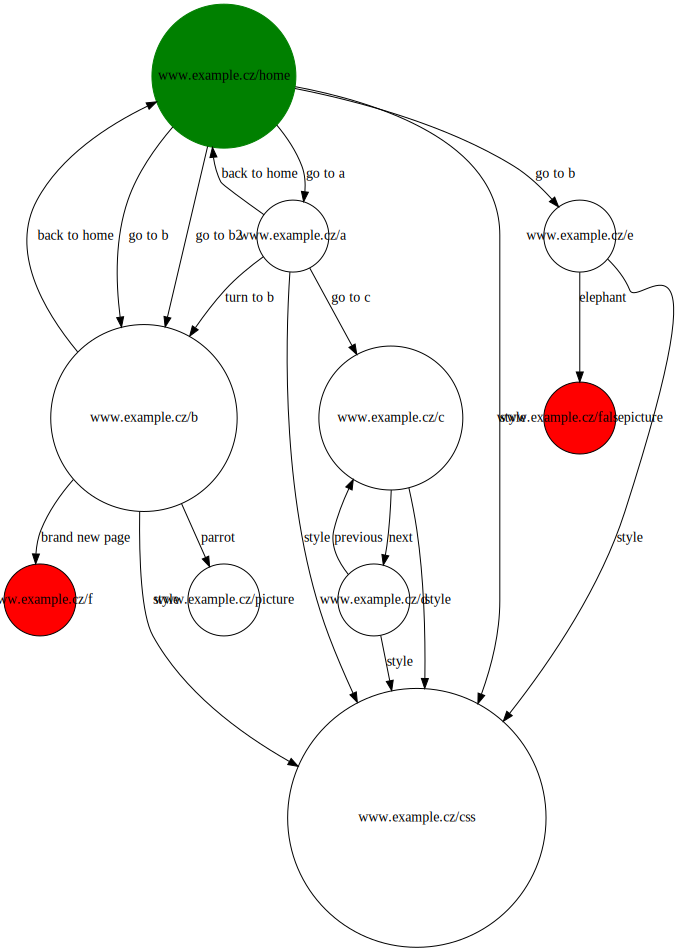
\includegraphics[width=0.8\textwidth]{pictures/graph.png}
		\caption{Graph results}
		\label{fig:graph}
\end{figure}

\subsubsection{Text graph result} \label{text}
This is the structured list of URL addresses crawled in this specific checkup. In the begging it is collapsed, but by clicking on underlined URL addresses with little arrow on theirs left side, you can easily click yourself through it and see how checked web presentation is organized and also where are invalid links, because they are here highlighted by red color and have theirs HTTP error code by left side. All this you can again see in the picture bellow.

\begin{figure}[H]
    \centering
    \includegraphics[width=0.8\textwidth]{pictures/text.png}
		\caption{Text graph result}
		\label{fig:text}
\end{figure}

\subsubsection{Graphical graph result} \label{graphical}
This is the graphical representation of URL addresses crawled in this specific checkup and its presented by oriented graph. All the nodes represent URL addresses, are also clickable, and by theirs colors you can also recognize, which of them are invalid. The edges then represents the specific way of the connection between two URL addresses displayed by nodes. More about these graph you can read here \url{http://en.wikipedia.org/wiki/Directed_graph} a example of the one is also here bellow.

\begin{figure}[H]
    \centering
    \includegraphics[width=0.8\textwidth]{pictures/graphical.png}
		\caption{Graphical graph result}
		\label{fig:graphical}
\end{figure}

\end{document}
